\documentclass{llncs}
\usepackage{amssymb}
\usepackage{url}
\usepackage{graphicx}

\title{Evaluation of GUHA Mining with Background Knowledge}
\author{Martin Ralbovsk\'{y}}
\institute{Department of Information and Knowledge Engineering,\\
University of Economics, Prague, W. Churchill Sq.~4, 130 67 Praha~3, Czech Republic
\\\email{martin.ralbovsky@gmail.com}}

\begin{document}
\maketitle

\begin{abstract}
Background knowledge is used for evaluation of specific KDD technique --
GUHA method. This is done by verification of verbal background knowledge
rules on a medical STULONG dataset. Formalization for the verbal rules
was developed and tools for verification of the rules against output of
GUHA procedures implemented. We conducted experiments that and drew 
conclusions about the mostly used settings of GUHA procedures. 
\end{abstract}

{\small {\bf Keywords:} Background knowledge, GUHA Method, STULONG dataset}

\section{Introduction}
Process of knowledge discovery in databases
(KDD) can be affected by using domain knowledge. 
In \cite{Ontology} authors identify four KDD stages where proper domain knowledge 
(ontologies) can be helpful: data understanding,
task design, result interpretation and result dissemination over the semantic web. 
In this work, we are
interested in evaluation of KDD techniques with respect to the used domain
knowledge and examined data. The evaluation should help to improve the task design
and result interpretation KDD stages. 

We are using the STULONG\footnote{\url{http://euromise.vse.cz/stulong}}
database as the examined data. The STULONG database
is an extensive epidemiological study of atherosclerosis primary prevention and was
examined also in \cite{Ontology}. Besides the data, STULONG contains some
domain knowledge examples created by medical experts. 
The knowledge (here named \emph{background knowledge}) consists of verbal rules
expressing relationships between two entities in the domain.

Because of the fact, that most of the data mining analysis
with STULONG were done with tools implementing GUHA method, we chose this
method to be evaluated by the background knowledge. By evaluation we mean
constructing various data mining tasks that should approve or disapprove
the background knowledge in the STULONG data and drawing conclusions from
the results of the tasks. We invented a formalization of verbal background
knowledge rules and implemented automatic tools to verify them against the
outputs of GUHA mining tasks. To our best knowledge, this work is the first
work to evaluate GUHA mining on bases of comprehensive background knowledge
verification.

The work is structured as follows: section \ref{section:guha} describes the GUHA method,
GUHA procedures used in this work and also recent tools implementing the method.
Section \ref{section:knowledge} explains background knowledge used, new 
formalization of the background knowledge and example of the formalization. 
Section \ref{section:experiments} shows conducted experiments and evaluates the GUHA method
on basis of the experiments. Section \ref{section:related} puts the work into context
of other works dealing with background knowledge and section~\ref{section:conclusion} concludes
the work and gives ideas about future research.

\section{The GUHA Method}
\label{section:guha}

GUHA method is one of the first methods of exploratory data analysis, developed in 
the mid-sixties in Prague. It is a general mainframe for retrieving interesting
knowledge from data. The method has firm theoretical foundations based on 
observational calculi and statistics \cite{GUHA2}. For purpose of 
this work let us explain only the basic principles of the method, as shown in 
Figure \ref{fig:GUHA}.

\begin{figure}[ht]
\centering
\mbox{\resizebox{45mm}{!}{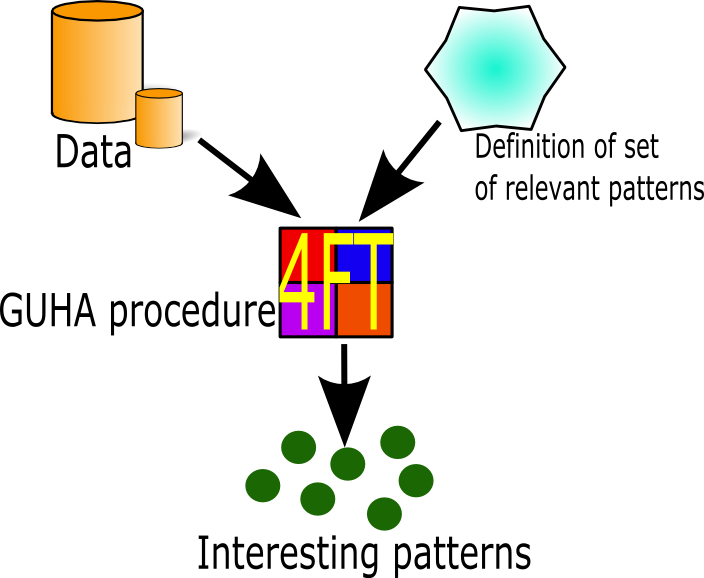
\includegraphics{GUHA.png}}}
\caption{The GUHA method}
\label{fig:GUHA}
\end{figure}

GUHA method is realized by GUHA procedures such as 4FT procedure to be described, 
located in the middle of the figure. Inputs of the procedure are data and a simple definition
of a possibly large set of relevant patterns. The procedure automatically generates
all the relevant patterns and verifies them against the provided data. Patterns that
are true are output of the procedure. In this work, we use procedure 4FT (described in
section \ref{section:4ft}) and procedure KL (described in section \ref{section:kl}).

\subsection{Procedure 4FT}
\label{section:4ft}

Classical \emph{apriori} \cite{Agrawal1} association mining searches rules in form 
$X \longrightarrow Y$, where 
$X$ and $Y$ are sets of items. Procedure 4FT searches (in the simplified form) for 
generalized association rules in form \mbox{$\varphi \approx \psi$}, 
where $\varphi$ and $\psi$ are 
\emph{Boolean attributes} and $\approx$ is a \emph{4ft-quantifier}. 
Relation \mbox{$\varphi \approx \psi$} is evaluated on the
basis of \emph{4ft table}, as shown in Table \ref{table:4FTcontingency}.

The term \emph{Boolean attribute} uses attributes. We use the 
term attribute in the sense of \emph{categorial attribute}, i.e.
attribute with finite number of values. Let A be an attribute, 
A = $\{a_{1}, a_{2}...a_{n}\}$ and $\alpha\subset A$, $\alpha\neq\emptyset$. 
Then $A(\alpha)$ is a \emph{basic Boolean attribute}.

Each \emph{basic Boolean attribute} is a \emph{Boolean attribute}.
If $\alpha$ and $\beta$ are \emph{Boolean attributes}, $\alpha\wedge\beta$, 
$\alpha\vee\beta$ and $\neg\alpha$ are \emph{Boolean attributes}.

\begin{table}[ht]
	\begin{center}
		\begin{tabular}{r|c|c}
		{\b M}        & $ \psi $ &  $ \neg \psi $ \\
		\hline
		     $  \varphi $  &  \ \ $ a  \ \ $    & $  \ \ b \ \  $    \\
		\hline
		   $ \neg \varphi $  &  $ c $    & $ d $    \\
		\end {tabular}
	\end{center}
	
	\begin{center}
	Table 1: 4ft table
	\end{center}
	\caption{4FT contingency table}
	\label{table:4FTcontingency}
\end{table}

A \emph{4ft table} is a quadruple of natural numbers 
\emph{$\langle$a, b, c, d$\rangle$}
so that:

\begin{itemize}
	\item \emph{a}: number of objects (rows of \emph{M}) satisfying $\varphi$ and $\psi$
	\item \emph{b}: number of objects (rows of \emph{M}) satisfying $\varphi$ and not 
	satisfying $\psi$
	\item \emph{c}: number of objects (rows of \emph{M}) not satisfying $\varphi$ but 
	satisfying $\psi$
	\item \emph{d}: number of objects (rows of \emph{M}) satisfying neither $\varphi$ nor $\psi$
\end{itemize}

\emph{4ft-quantifier} expresses kind of dependency between $\varphi$ and $\psi$.
The quantifier is defined as a condition over the 4ft table. In this 
work, we use the two most common 4ft-quantifiers: \emph{founded implication}
and \emph{above average dependence}.

\medskip
The \emph{founded implication} is the basic quantifier for the 4FT procedure.
It is defined by the following condition:
$$a \geq Base \wedge \frac{a}{a+b} \geq p$$
where \emph{Base} and \emph{p} are threshold parameters of the procedure. The
\emph{Base} parameter represents absolute number of objects that satisfies 
$\varphi$. In our work we will use relative \emph{Base} representation, 
$\frac{a}{a+b+c+d}$. The \emph{Base} parameter corresponds to the 
\emph{support} and \emph{p} to the \emph{confidence} parameters 
of classical association mining.

\medskip
The \emph{above average dependence} is defined by the following condition:
$$\frac{a}{a+b}\geq(p)\frac{a+c}{a+b+c+d} \wedge a \geq Base$$
where $p$ and $Base$ are user-defined parameters\footnote{The $p$ parameter
is originally defined in \cite{Rauch} as $\frac{a}{a+b}\geq(1+p)\frac{a+c}{a+b+c+d}$.
We alter this definition in order to avoid negative $p$ results in the experiments.}.
Again, we will use the
relative \emph{Base} representation $\frac{a}{a+b+c+d}$. So, the quantifier 
can be verbally interpreted as
\emph{"among object satisfying $\varphi$, there are at least p per cent 
more objects satisfying $\psi$ then among all observed objects and there are
at least Base per cent of observed objects satisfying $\varphi$ and $\psi$".}

\subsection{Procedure KL}
\label{section:kl}
Procedure KL \cite{KL} searches (in the simplified form) for rules 
in form $R \sim C$, where $R$ and $C$ are categorial attributes.
The symbol $\sim$ is called \emph{KL-quantifier}. The rule $R \sim C$ means, 
that categorial attributes $R$ and $C$ are in relation described by 
$\sim$. In this work, we are using the \emph{Kendall's quantifier}.

\medskip
\emph{Kendall's quantifier} is based on \emph{Kendall's coefficient} 
$\tau_{b}$\cite{Kendall}. It is defined as

$$\tau_{b}=\frac{2(P-Q)}{\sqrt{(n^{2}-\sum_{k}n^{2}_{k,*})(n^2-\sum_{l}n^{2}_{*,l})}}$$
where
$$P=\sum_{k}\sum_{l}n_{k,l}\sum_{i>k}\sum_{j>l}n_{i,j},Q=\sum_{k}\sum_{l}n_{k,l}\sum_{i>k}\sum_{j<l}n_{i,j}$$
$\tau_{b}$ ranges from $\left\langle -1,1\right\rangle$, where values $\tau_{b}>0$
indicate positive ordinal dependence\footnote{High values of $C$ often coincide with
high values of $R$, low values of $C$ often coincide with low values of $R$.}, values
$\tau_{b}<0$ negative ordinal dependence, $\tau_{b}=0$ ordinal independence and 
$|\tau_{b}|=1$ functional dependence of $C$ on $R$. In this work, we are using the
Kendall's quantifier to construct \emph{abstract quantifiers} discussed in 
section \ref{section:types}.

\subsection{GUHA Tools}
Apart from the tools presented in this section, several systems implementing
GUHA procedures were developed in the past. In recent years, the
\emph{LISp-Miner} system has been the most significant GUHA tool. This system
has been under development since 1996 at the University of Economics, Prague.
It includes six GUHA procedures including procedure KL and lighter version
of 4FT procedure \cite{Ralbovsky} in addition to other data preparation and 
result interpretation modules.

In 2004, the Ferda project started as an initiative to build a new
visual data mining successor of the \emph{LISp-Miner} system. Creators 
(at the Faculty of Mathematics and Physics, 
Charles University, Prague) succeeded in developing an user friendly
visual system with advanced features such as high level modularity, support
for distributed computing or reusability of the task setting \cite{Ferda}.
At present there are several research activities taking advantage of the system.
Figure \ref{fig:Ferda} shows the Ferda working environment. For purposes of
this work, there were modules implemented in the Ferda system as well.

\begin{figure}[ht]
\centering
\mbox{\resizebox{110mm}{!}{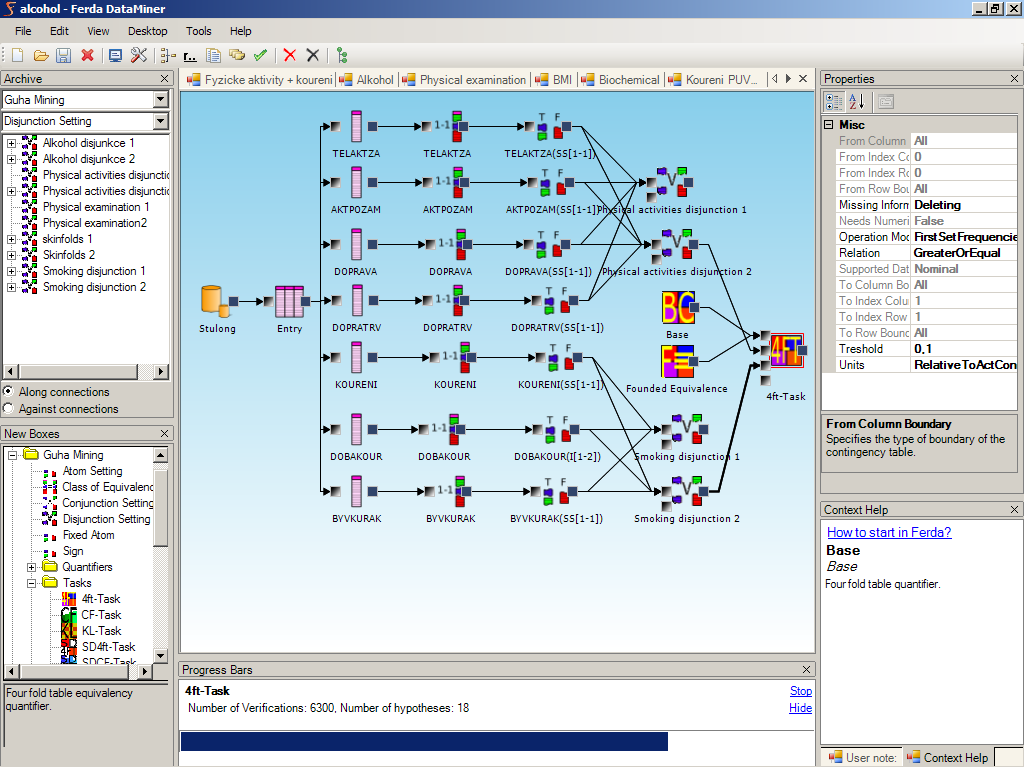
\includegraphics{Ferda.png}}}
\caption{Ferda environment}
\label{fig:Ferda}
\end{figure}

\section{Background Knowledge}
\label{section:knowledge}

\subsection{Considered Background Knowledge Types}
\label{section:types}
Background knowledge (also \emph{field knowledge} or \emph{prior knowledge}) 
is knowledge that comes from the user or a community of users and integrates 
knowledge, which the community can agree upon and consider it common. Various
fields of KDD define background knowledge differently, there is no central
theory for the term. In the context of GUHA mining,
we think of background knowledge as a part of domain knowledge,
knowledge that is specific to particular domains (medicine, chemistry, etc.).
We define background knowledge as a set of various verbal rules that
are accepted in a specific domain as a common knowledge\footnote{Note the
difference between our vague definition and precise definitions e.g. in ILP}. 
The rule can describe functional dependence between quantities, relationship
between entities or say something about their behavior. Below are presented
example rules taken from STULONG\footnote{The study (STULONG) was realized at the
2nd Department of Medicine, 1st Faculty of Medicine of Charles University and 
Charles University Hospital, U nemocnice 2, Prague 2 (head. Prof. M. Aschermann, 
MD, SDr, FESC), under the supervision of Prof. F. Boud\'{i}k, MD, ScD, with collaboration 
of M. Tome\v{c}kov\'{a}, MD, PhD and Ass. Prof. J. Bultas, MD, PhD. The data were transferred 
to the electronic form by the European Centre of Medical Informatics, Statistics and Epidemiology of Charles University and Academy of Sciences (head. Prof. RNDr. J. 
Zv\'{a}rov\'{a}, DrSc). The data resource is on the web pages \url{http://euromise.vse.cz/challenge2004}. 
At present time the data analysis is supported by the grant of the Ministry of 
Education CR Nr LN 00B 107.}: 

\begin{itemize}
\item If education increases, wine consumption increases as well.
\item Patients with greater responsibility in work tend to drive to work by car.
\end{itemize}

\subsection{Background Knowledge Formalization}
\label{section:formalization}
In order to automatically verify background knowledge against the data, a new formalization
needed to be thought out. 
Background knowledge contains heterogeneous verbal formulations of dependences
and relationships in the domain. The relevance and validity of the formulations varies:
the relationships in physics are formed exactly by mathematical equations, but for
example in sociology they mean only expected behavior or opinion of a group of people.
Our aim is to find formalization usable for both domains.

We present a new \emph{Formalization with attributes, validation literals and 
abstract quantifiers} first used in \cite{Diplomka}. The main idea behind the
formalization is to make it as close to GUHA terms as possible while still
enabling large expressive possibilities of the verbal rule. Because of shorter
format of the article, we present only an overview and an example of the new
formalization with a little reasoning. The topic is fully covered in 
\cite{Diplomka}, section 3.2.2.

\medskip
\emph{Attribute} is the basic term for the new formalization. \emph{Attribute}
is defined as a result of domain categorization and is used
to create \emph{categorial attributes}, inputs of the \emph{KL} procedure.

\medskip
\emph{Validation literal} is a special type of \emph{literal} used to express
background knowledge. \emph{Literal} is a basic Boolean 
attribute or its negation. We define the \emph{literal length}
as the size of the categories' subset. \emph{Validation literal} is a literal,
which has \emph{literal length} equal to 1.

\medskip
\emph{Abstract quantifier} is a generalization of a quantifier or quantifiers of 
a procedure (4FT or KL). The idea behind abstract quantifiers
is to create a "black-box" quantifier: user does not need to fill any numeral 
parameters of the quantifier. The quantifier is then more suitable for transferring
verbal background knowledge rules into formalized form.

\subsection{Formalization Example}
With all the terms explained, let us see how the formalization is applied to 
a specific verbal rule \textbf{If education increases, wine consumption increases as well.}
as presented in Section~\ref{section:types}. The rule defines relationship
between two measurable quantities of a patient. These quantities are stored in the
database in the form of columns of a table, so attributes can be created.
We name the attributes for \textbf{education} and \textbf{wine consumption}
\emph{education} and \emph{wine} respectively.

For this paragraph we will consider only the KL procedure. 
The procedure searches (in the simplified form) for rules 
in form $R \sim C$, where $R$ and $C$ are categorial attributes, which
derive from attributes.
When \textbf{education} and \textbf{wine consumption}
out of the rule are to be formalized with \emph{R} and \emph{C} of the hypothesis,
then the part \textbf{If ... increases, ... increases as well} could be formalized with
a proper abstract quantifier. We call this quantifier
\emph{increasing dependence} and is implemented as a special setting of the 
Kendall quantifier (to be described later). With all the knowledge
stated above, the rule \textbf{If education increases, wine consumption increases
as well} can be formally written as \emph{education} $\uparrow$ \emph{wine}, where
$\uparrow$ states for increasing dependence abstract quantifier.

We can also define the formalization for the 4FT procedure. The hypotheses
of this procedure consist of Boolean attributes, therefore it is better to use validation literals. If we presume correct categorization, out of
\emph{attributes education} and \emph{wine} the \emph{validation literals
education(HIGH)} and \emph{wine(HIGH)} can be created. Similarly
to KL formalization we can use abstract quantifier to 
note the dependence. Then the rule \textbf{If education increases, wine consumption
increases as well} can be formalized as \emph{education(HIGH)} $\Rightarrow$
\emph{wine(HIGH)} with a proper abstract quantifier $\Rightarrow$

Formalization with the 4FT procedure cannot consider the whole \emph{attributes}
but only some of its categories, thus it is weaker. However there may be situations 
when it is feasible to use the 4FT procedure. If the examined attribute is not
ordinal, the KL procedure cannot be used. Also there may be ordinal attributes
with such a small number of categories, that is preferred to use 4FT 
procedure (which was often the case in our experiments).

In the beginning of section \ref{section:formalization}, a requirement was given on the formalization
to be able to represent various kinds of relationships between the
entities of the domain. The formalization with attributes, validation 
literals and abstract quantifiers fulfills this requirement, because the
formalization does not pose any restrictions on the relationships - 
the relationship is expressed by the abstract quantifier. 

\section{Experiments}
\label{section:experiments}
The main reason for constructing a formalization was to experimentally 
find out, if background knowledge gained from domain experts is apparent 
in the data by GUHA means. This part of the paper gives information about experiments:
section \ref{section:setup} describes experiments' setup, 
sections \ref{section:default} and \ref{section:suitable} show two conducted
experiments and section \ref{section:findings} evaluates the results of the
experiments. 

\subsection{Setup}
\label{section:setup}
Modules of the Ferda system were created for purposes of this work and of work
\cite{Diplomka}. The modules enable the formalization with attributes,
validation literals and abstract quantifiers setting. They also automatically
find rules from the output of 4FT and KL procedures that match the formalized 
background knowledge. The details of the implementation, with proper 
explanation of the modules and description of algorithms can be found 
in \cite{Diplomka}.

Special attention was paid to selection of abstract quantifiers. For the 
KL procedure, we chose variations of Kendall quantifier named 
\emph{increasing} and \emph{decreasing dependence} for observing positive and
negative ordinal dependence. Out of many 4ft-quantifiers, we chose the
two most used quantifiers introduced in section \ref{section:4ft}, the
founded implication and above average dependence. We presumed
that if they are most used, they should be somehow "good". 

We chose 8 sample rules constructed by medical experts
concerning education and responsibility
in work. These rules were selected as a sample of the rules that can be mined upon
(without changing the database schema). Rules are listed in Table \ref{tab:rules}. 
We used the same common categorization of STULONG attributes both for the task
settings and for the formalization settings.

\begin{table}[ht]
	\begin{tabular}{|p{1,5cm}|p{5cm}|p{5cm}|}
		\hline
			\textbf{Number} & \textbf{Rule - left side} & \textbf{right side}\\
		\hline
			\textbf{1} & If education increases & physical activity after work increases as well\\
		\hline
			\textbf{2} & If education increases & responsibility in work increases as well\\
		\hline
			\textbf{3} & If education increases & wine consumption increases as well\\
		\hline
			\textbf{4} & If education increases & smoking decreases\\
		\hline
			\textbf{5} & If education increases & physical activity in work decreases\\
		\hline
			\textbf{6} & If education increases & beer consumption decreases\\
		\hline
			\textbf{7} & Patients with greater responsibility in work & tend to drive to work by car\\
		\hline
			\textbf{8} & Patients with smaller responsibility in work & tend to use public transport to
			get to work\\
		\hline
	\end{tabular}
	\caption{Verified rules}
\label{tab:rules}
\end{table}

\subsection{Default Quantifiers' Settings}
\label{section:default}
There are threshold values of parameters defined for each quantifier, which tell
us when quantifier's output is significant. We call them \emph{default quantifiers'
settings}. These values were set up by an agreement among data mining experts.
The aim of the first conducted experiment was to verify, if there are in there are any 
rules verified with aid of formalization and abstract quantifiers defined in
previous section backing the background knowledge with default settings. 

We chose 0.7 and -0.7 value of the Kendall's coefficient for the
increasing and decreasing dependency abstract quantifiers respectively.
For the founded implication quantifier, the default values are 0.95 for
the $p$ parameter and 0.05 for the (relative) $Base$ parameter. For the
above average dependence quantifier, the default values are 1.2 for th
$p$ parameter and again 0.05 for the $Base$ parameter.

\begin{table}[ht]
	\centering
	\begin{tabular}{|p{2,5cm}|p{1cm}|p{1cm}|p{1cm}|p{1cm}|}
		\hline
		\textbf{Rule number}&\textbf{ID}&\textbf{DD}&\textbf{FI}&\textbf{AA}\\
		\hline
		1&YES&x&NO&NO\\
		\hline
		2&YES&x&NO&NO\\
		\hline
		3&NO&x&YES&NO\\
		\hline
		4&x&NO&NO&NO\\
		\hline
		5&x&NO&NO&YES\\
		\hline
		6&x&NO&NO&NO\\
		\hline
		7&x&x&NO&NO\\
		\hline
		8&x&x&NO&NO\\
		\hline
	\end{tabular}
\caption{Verification of quantifier's settings}
\label{tab:validation1}
\end{table}

Table~\ref{tab:validation1} shows the results of the first experiment. The \textbf{ID},
\textbf{DD}, \textbf{FI} and \textbf{AA} stands for increasing dependence, 
decreasing dependence, founded implication and above average dependence
quantifiers. \textbf{YES} means that the rule was found with the given quantifier,
\textbf{NO} means that the rule was not found and \textbf{x} means that the
rule was not meaningful for the given quantifier.

Before we draw any conclusions from the experiment, let us first state some 
presumptions about the data source. The data table \emph{Entry}, which was mined 
upon, contains records about the entry examination of 1417 patients. Because of
this number, we consider the data to be statistically significant. We also
presume no errors in the data and proper categorization (described in \cite{Diplomka}). 
Finally, if we want to question settings of individual quantifiers, we
presume that the background knowledge rules are "somehow stored" in the data.
For example that the number of patients approving the background knowledge 
rule is greater then the number of patients disapproving the rule. 

The most interesting result of the experiment the disapproval of all the rules except
one with the founded implication and also the above average
quantifier. The fact leads to a conclusion that the $p$ parameters of 4FT quantifiers
are too restrictive, e.g. there should be 95\% confidence of the rule when
using founded implication quantifier. 

\subsection{Suitable Quantifiers' Settings}
\label{section:suitable}
As the previous section showed, the default settings of a quantifier can be
misleading. The next conducted experiment tries to find suitable quantifiers'
settings, based on the background knowledge rule validation. We gradually
decreased the $p$ settings of the founded implication and
above average dependence quantifiers. We did not experiment with the
KL quantifiers, because of the complexity of the problem\footnote{The 
results need not to improve merely by changing a parameter of a quantifier. 
We also need to take the shape of the KL contingency table into consideration.}.
With this technique, we could examine more background knowledge rules,
determine the value of the parameter for each rule and compute the average
of the values for each examined dataset. New mining with the quantifier can be
done with this average value and new relevant relationships in the data could
be discovered.

\begin{table}[ht]
	\centering
	\begin{tabular}{|p{2,5cm}|p{1,5cm}|p{1,5cm}|}
		\hline
		\textbf{Rule number}&\textbf{FI}&\textbf{AA}\\
		\hline
		1&0.83&1,03\\
		\hline
		2&0.72&0.43\\
		\hline
		3&1&0.68\\
		\hline
		4&0.32&1.17\\
		\hline
		5&0.28&1.34\\
		\hline
		6&0.38&1.17\\
		\hline
		7&0.16&1.15\\
		\hline
		8&0.64&1.07\\
		\hline
	\end{tabular}
\caption{Exact quantifiers values}
\label{tab:validation2}
\end{table}

As we can see in Table~\ref{tab:validation2}, the results of the experiment
are rather disappointing for the founded implication quantifier. Majority
of rules had the \emph{P} value below 0.5. We got better results for the 
above average dependence quantifier where the \emph{p} parameter was only twice below 1. 
However, only once the value exceeded the desired 1.2 value. 

\subsection{Evaluation}
\label{section:findings}
Considering the KL procedure, we obtained reasonable results for the increasing
dependence and bad results for the decreasing dependence abstract quantifiers.
This may be caused by the fact, that the categorial attributes $R$ and $C$ of the task setting contained few categories and thus irregularities of the  KL contingency table 
(see \cite{KL} for details) could easily affect the quantifier.

Considering the 4FT procedure, there results for above average dependence were
reasonable. On the other hand, the most used quantifier founded implication
did not prove to be useful at all. This may be caused by the fact, that for rules 
no. 4, 5 and 6 ($\varphi$ increasing,
$\psi$ decreasing) founded implication is not a suitable quantifier. 

Although the formal theory of the quantifiers (KL and 4FT) is well developed
\cite{Rauch}, our experiments showed that semantically sound interpretation is
yet to be researched. \cite{Kupka} is the first attempt of summarized semantic
explanation of significant quantifiers. 

\section{Related Work}
\label{section:related}

In \cite{Puppe}, authors use background knowledge for subgroup discovery.
Important part of the work tries to divide background knowledge into classes and deals
separately with each class. Unfortunately the rules and formalization defined in
this work does not belong to any of the classes defined.

In \cite{Faure}, authors developed ideologically similar approach: they used
classical association mining in cooperation with a Bayesian network to store
the knowledge from domain experts (here called \emph{a priori expert knowledge})
and improved both the association rules mining and the Bayesian
network in iterations. This approach is stronger from the methodological point of view 
(complex methodology is defined) and also enables revision of the domain expert
knowledge. However, our background knowledge formalization is less restrictive
than the Bayesian network and the GUHA procedures offer greater possibilities than
the classical association mining.

\cite{Qualitative2} show another formalization of background knowledge.
It is based on qualitative models and used for induction learning. This model is
not suitable for GUHA mining, mainly because the strict mathematical requirements
of the model. 

The data from STULONG itself have been matter of long run research 
\cite{Stulong2,Stulong4}. \cite{Adamek} deals with background
knowledge rules annotation into a attribute matrix. This annotation is a
simplification of our formalization without proper explanation of suggested
abstract quantifiers.

\section{Conclusion and Future Work}
\label{section:conclusion}
We focused on evaluation of specific KDD technique -- GUHA mining by verifying
background knowledge rules on a specific STULONG dataset. Background knowledge
consisted of verbal rules created by domain experts. These rules express
relationship between two entities of the domain. 

In order to automatically verify background knowledge rules, a formalization
of them needed to be developed. Our formalization with attributes, validation
literals and abstract quantifiers is tailored for the GUHA method, more specifically
their 4FT and KL procedures. We also developed automatic tools for the verification
of formalized background knowledge rules against the output of the two GUHA
procedures. 

Experiments were conducted testing background knowledge rules from the STULONG dataset
against the data. In the first experiment, we tried to verify background knowledge
against default settings of mostly used quantifiers. We found default settings of
the quantifiers too strict. Then we continued to find out which values of quantifiers'
parameters can verify the background knowledge rules. Results of this experiment were
reasonable for the above average dependence quantifier but disappointing for the
founded implication quantifier. 

The overall output of the experiments is, that more attention should be paid to
semantic interpretation of quantifiers and their default settings. This should
be the main direction for the future work in the field. New abstract quantifiers
need to be defined and conditions for their usage investigated. This requires
cooperation between the domain experts and data miners. One of the possible
improvements helping to better reflect real life situations is enabling
fuzzy quantifiers and attributes. 

\section*{Acknowledgment}

This work was supported by the project MSM6138439910 of the
Ministry of Education of the Czech Republic, project IG407056 of University
of Economics, Prague and by the project 201/05/0325 of the Czech Science
Foundation. 

We would like to thanks our research colleagues Jan Rauch and Vojt\v{e}ch 
Sv\'{a}tek for help, valuable comments and reviews.

\begin{thebibliography}{20}

\bibitem{Agrawal1}
Agrawal R., Imielinski T., Swami A.:
\emph{Mining association rules between sets of items in large databases}.
Proc. of the ACM SIGMOD Conference on Management of Data, p.~207~--~216

\bibitem{Puppe}
Atzmueller M., Puppe F.: \emph{A Methodological View on Knowledge-Intensive Subgroup
Discovery}. In: S. Staab and V. Sv\'{a}tek (Eds.): EKAW 2006, LNAI 4248, 
Springer-Verlag 2006, p.~318~--~325

\bibitem{Stulong2}
Berka P., Tome\v{c}kov\'{a} M., Rauch J.: \emph{The ECML/PKDD Discovery Challenge on the Atherosclerosis Risk Factors Data}. In: Popel\'{i}nsk\'{y} L., Kr\'{a}tk\'{y} M. (ed.): Znalosti 2005. Ostrava, V�B TU Ostrava 2005, pp. 18�-28. ISBN 80-248-0755-6.

\bibitem{Faure}
Faur\'{e} C., Delpart S., Boulicaut J., Mille A.: \emph{Iterative Bayesian Network
Implementation by Using Annotated Association Rules}. In: S. Staab and V. Sv\'{a}tek
(Eds.): EKAW 2006, LNAI 4248, Springer-Verlag 2006, p.~326~--~333

\bibitem{GUHA2}
H\'{a}jek P., Havr\'{a}nek, T.: \emph{Mechanising Hypothesis
Formation - Mathematical  Foundations  for  a   General  Theory}.
Springer-Verlag: Berlin  - Heidelberg - New York, 1978.

\bibitem{Ferda}
Kov\'{a}\v{c} M., Kucha\v{r} T., Kuzmin A., Ralbovsk\'{y} M.: \emph{Ferda, 
New Visual Environment for Data Mining}. Znalosti 2006, 
Conference on Data Mining, Hradec Kr\'{a}lov\'{e} 2006,p.~118~--~129 (in Czech)

\bibitem{Kupka}
Kupka D.: \emph{User support 4ft-Miner procedure for Data Mining}. Master Thesis,
Faculty of Mathematics and Physics, Charles University, Prague 2006 (in Czech)

\bibitem{Stulong4}
Lucas N., Az\'{e} J.. Sebag M.: \emph{Atherosclerosis Risk Identification and Visual Analysis}. In Berka, P. (ed.): Discovery Challenge Workshop Notes. ECML/PKDD-2002. Helsinki 2002.

\bibitem{Qualitative2}
Matwin S., Rouge T.: \emph{Explainable Induction with an Imperfect Qualitative Model}.
\url{http://citeseer.ist.psu.edu/matwin95explainable.html}

\bibitem{Diplomka}
Ralbovsk\'{y} M.: \emph{Usage of Domain Knowledge for Applications of GUHA
Procedures}, Master Thesis, Faculty of Mathematics and Physics, Charles University,
Prague 2006 (in Czech)

\bibitem{Ralbovsky}
Ralbovsk\'{y} M., Kucha\v{r} T.: 
\emph{Using Disjunctions in Association Mining}. 
In: Perner P.: Advances in Data Mining, Springer-Verlag 2007, to appear

\bibitem{Rauch}
Rauch J.: \emph{Logic of Association Rules}. In: Applied Inteligence, Vol. 22,
Issue 1, p.~9~--~28

\bibitem{KL}
Rauch J., \v{S}im\accent23unek M., L\'{i}n V.:
\emph{Mining for Patterns Based on Contingency Tables by KL-Miner � First
Experience}.
In: Lin T.Y. (ed.): Foundations and Novel Approaches in Data Mining. Springer-Verlag,
pp. 155--167

\bibitem{Adamek}
Rauch J., Tome\v{c}kov\'{a} M.: \emph{System of Analytical Questions and
Reports on Mining in Health Data -- a Case Study}. Submitted to IADIS 2007

\bibitem{Kendall}
\v{R}eh\'{a}k J., \v{R}eh\'{a}kov\'{a} B.: \emph{Analysis of Categorized Data
in Sociology} (in Czech). Academia: Prague, Czechoslovakia, 1986

\bibitem{Ontology}
Sv\'{a}tek V., Rauch J., Ralbovsk\'{y} M.: \emph{Ontology-Enhanced Association
Mining}. In: Ackermann, Berendt (eds.). Semantics, Web and Mining, 
Springer-Verlag, 2006

\end{thebibliography}

\end{document}